\chapter{Grundlagen}
\section{Einführung in eingebettete Systeme}
\subsection{Definition}
Eingebettete Systeme sind informationsverarbeitende Systeme, die in umgebende Produkte integriert sind \cite {Marwedel.2021}. Sie sind aus unserem Alltag nicht mehr wegzudenken und bilden die Grundlage moderner Technologien. Je nach Schwerpunkt ergibt sich eine leicht unterschiedliche Definition:  
\begin{itemize}
    \item Marwedel definiert eingebettete Systeme als \glqq informationsverarbeitende Systeme, die in umgebende Produkte integriert sind.\grqq\cite{Marwedel.2021}.
    \item In der englischen Literatur wird der Fokus auf die Software gelegt: \glqq Embedded software is software integrated with physical processes. The technical problem is managing time and concurrency in computational systems.\grqq\cite{Marwedel.2021}.
    \item Die dritte Definition betont die Interaktion mit der Umgebung: \glqq Cyber-physikalische Systeme (engl. Cyber-Physical Systems (CPS)) bestehen aus der Integration von Berechnungen und physikalischen Prozessen.\grqq\cite{Marwedel.2021}.
\end{itemize}  

Die verschiedenen Definitionen zeigen, dass eingebettete Systeme nicht nur aus Hardware bestehen, sondern auch eine enge Verzahnung mit Software und physikalischen Prozessen aufweisen.  

\subsection{Eingebettete Systeme und Cyber-physikalische Systeme (CPS)}
Ein Cyber-physikalisches System (CPS) kann als eine Weiterentwicklung eingebetteter Systeme betrachtet werden. Während eingebettete Computersysteme den Fokus auf die informationsverarbeitende Einheit legen, erweitert ein CPS diesen Ansatz durch die Integration von Netzwerken und Echtzeit-Interaktionen mit der Umgebung \cite{Marwedel.2021}.  

Die folgende Abbildung \ref{fig:cbs-systeme} visualisiert die Architektur eines CPS. Solche Systeme kombinieren eingebettete Computersysteme mit Netzwerken, um physikalische Prozesse zu steuern und Daten in Echtzeit auszutauschen. Dies macht sie zu einem zentralen Element der Industrie 4.0 \cite{Westermann.2016}.  
CPS ermöglichen intelligente, vernetzte und automatisierte Systeme, die in vielen Branchen – von der Automobilindustrie bis zur Medizintechnik – eingesetzt werden \cite{Westermann.2016}. Eingebettete Systeme, eingebettete Computersysteme und CPS sind somit eng miteinander verbunden, wobei CPS die umfassendste Form darstellen.  

\begin{figure}[h]
	\centering
	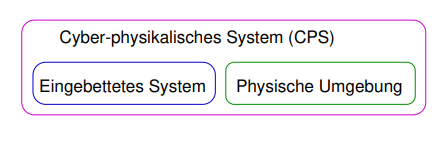
\includegraphics[width=0.9\textwidth]{img/CPS.png}
	\caption{Abbildung zu CPS \cite{Marwedel.2021}}
	\label{fig:cbs-systeme}
\end{figure}
Die Definitionen eingebetteter Systeme können zu Beginn für den Leser schwer verständlich sein. Daher wird im Folgenden eine zusätzliche Erklärung zu eingebetteten Systemen gegeben.  

Historisch war die Informationsverarbeitung eng mit Großrechnern und großen Bandlaufwerken verbunden. Die Miniaturisierung der Technologie führte jedoch zur Einführung von Personal Computern (PCs), die zunächst primär für Büroanwendungen eingesetzt wurden \cite{Ubiquitous_Computing_1994}. Parallel dazu entstanden Rechner, die speziell für Steuerungs- und Regelungsaufgaben in physischen Systemen konzipiert wurden \cite{Ubiquitous_Computing_1994}.  

Mark Weiser prägte später den Begriff des „allgegenwärtigen Rechnens“ (ubiquitous computing). Er prognostizierte, dass Computer und Informationen zukünftig jederzeit und überall verfügbar sein würden und dass Computer so in Produkte integriert würden, dass sie für den Nutzer unsichtbar sind \cite{Ubiquitous_Computing_1994}. Diese Entwicklung führte zur Einführung des Konzepts des „unsichtbaren Computers“. Beispiele hierfür sind unter anderem Fernbedienungen, Kameras oder Mobiltelefone.  

Verwandte Konzepte sind das \textbf{durchdringende Rechnen} (pervasive computing) und die \textbf{umgebende Intelligenz} (ambient intelligence). Diese Begriffe betonen unterschiedliche Aspekte der modernen Informationstechnologie:  
\begin{itemize}
    \item \textbf{Allgegenwärtiges Rechnen}: Ziel ist es, Informationen jederzeit und überall bereitzustellen \cite{Ubiquitous_Computing_1994}.  
    \item \textbf{Durchdringendes Rechnen}: Fokussiert sich auf die praktische Anwendung und Nutzung vorhandener Technologien \cite{Ubiquitous_Computing_1994}.  
    \item \textbf{Umgebende Intelligenz}: Bezieht sich auf die Nutzung von Informationstechnologie, beispielsweise in intelligenten Wohnhäusern oder Bürogebäuden \cite{Ubiquitous_Computing_1994}.
\end{itemize}  

Viele dieser Konzepte sind mittlerweile Realität geworden, insbesondere durch die Verbreitung kleiner mobiler Geräte und des mobilen Internets, das zahlreiche Bereiche des täglichen Lebens beeinflusst. Darüber hinaus wird die Künstliche Intelligenz künftig eine zentrale Rolle in der Weiterentwicklung dieser Technologien spielen. Auf diesen Aspekt wird später eingegangen.  

Ein weiterer wesentlicher Bestandteil eingebetteter Systeme ist der Kommunikationsaspekt. Abbildung \ref{fig:kommunikation} illustriert die Beziehung zwischen Kommunikation und eingebetteten Systemen.  
\begin{figure}[h]
	\centering
	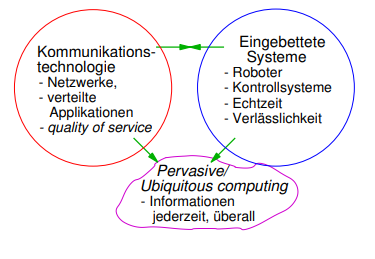
\includegraphics[width=0.9\textwidth]{img/kommunikation.png}
	\caption{Kommunikation und eingebettete Systeme \cite{Marwedel.2021}}
	\label{fig:kommunikation}
\end{figure}
Die "National Science Foundation" (NSF) in den USA hebt die Bedeutung der Vernetzung und Kommunikation verteilter Systeme im Kontext Cyber-physikalischer Systeme (CPS) hervor. In deutscher Übersetzung wird festgestellt, dass diese aufkommenden Systeme „koordiniert, verteilt und verbunden sein werden und dass sie robust und reaktionsfähig sein müssen“ \cite{Council.2015}.  

Cyber-physikalische Systeme stellen eine Weiterentwicklung eingebetteter Systeme  dar. Während eingebettete Systeme meist isoliert und spezialisiert für spezifische Aufgaben entwickelt werden, zeichnen sich CPS durch ihre umfassende Vernetzung und die Integration physischer und digitaler Prozesse aus \cite{Marwedel.2021}. Eingebettete Systeme agieren hauptsächlich lokal und reaktiv, ohne größere Datenanalysen oder Interaktionen mit anderen Systemen durchzuführen \cite{Marwedel.2021}. CPS hingegen sind proaktiv, verteilt und in der Lage, Daten in Echtzeit zu verarbeiten und Entscheidungen zu treffen, um komplexe und dynamische Aufgaben zu bewältigen \cite{Marwedel.2021}. Diese Eigenschaften machen CPS zu einem unverzichtbaren Bestandteil moderner Anwendungen, die zunehmend auf Vernetzung und Automatisierung angewiesen sind.  

Diese Aussage verdeutlicht die Anforderungen an moderne CPS, die nahtlose Kommunikation und Kooperation gewährleisten müssen, selbst wenn sie über unterschiedliche geografische Standorte verteilt sind. Solche Systeme müssen nicht nur zuverlässig (robust) arbeiten, sondern auch in der Lage sein, auf Veränderungen in ihrer Umgebung schnell und flexibel zu reagieren \cite{Council.2015}.  

Diese Eigenschaften sind essenziell für die erfolgreiche Integration von CPS in verschiedenen Anwendungsbereichen, wie etwa in der Automobilelektronik, der Robotik, intelligenten Gebäuden, dem Gesundheitswesen, der Agrartechnik, der öffentlichen Sicherheit oder dem Maschinenbau \cite{Westermann.2016, Council.2015, Wang.2021}.
